\documentclass{article} % Класс печатного документа

\usepackage{hyperref} % Для вставки гиперссылок
\usepackage{listings} % Для вставки кусков кода
\usepackage{graphicx} % Вставка изображений
\usepackage[utf8]{inputenc} % Кодировка исходного текста - utf8
\usepackage[english,russian]{babel} % Поддержка языка - русского с английским
\usepackage{indentfirst} % Отступ в первом абзаце

\title{Отчёт 7\protect\\Дескриптивная статистика и регрессия} % Заголовок документа
\author{Свичкарев А.\,В.} % Автор документа
\date{\today} % Текущая дата

\begin{document} % Конец преамбулы, начало текста

\maketitle % Печатает заголовок, список авторов и дату

\section{Задание №1}
Функции реализованы с помощью библиотек \verb$math$ и \verb$numpy$:
\lstinputlisting[language=Python, firstline=1, lastline=25]{../code7.py}

В секции Исходный код представлены тесты и ожидаемые результаты на указанной в задание выборке.

\section{Задание №2}
\lstinputlisting[language=Python, firstline=28, lastline=38]{../code7.py}

В секции Исходный код представлены тесты и ожидаемые результаты на указанной в задание выборке.

\section{Задание №3}
\lstinputlisting[language=Python, firstline=41, lastline=45]{../code7.py}

В секции Исходный код представлен тест линейной регрессии с фиксированными значениями псевдо-генеротора чисел.

\section{Задание №4}
\noindent\makebox[\textwidth]{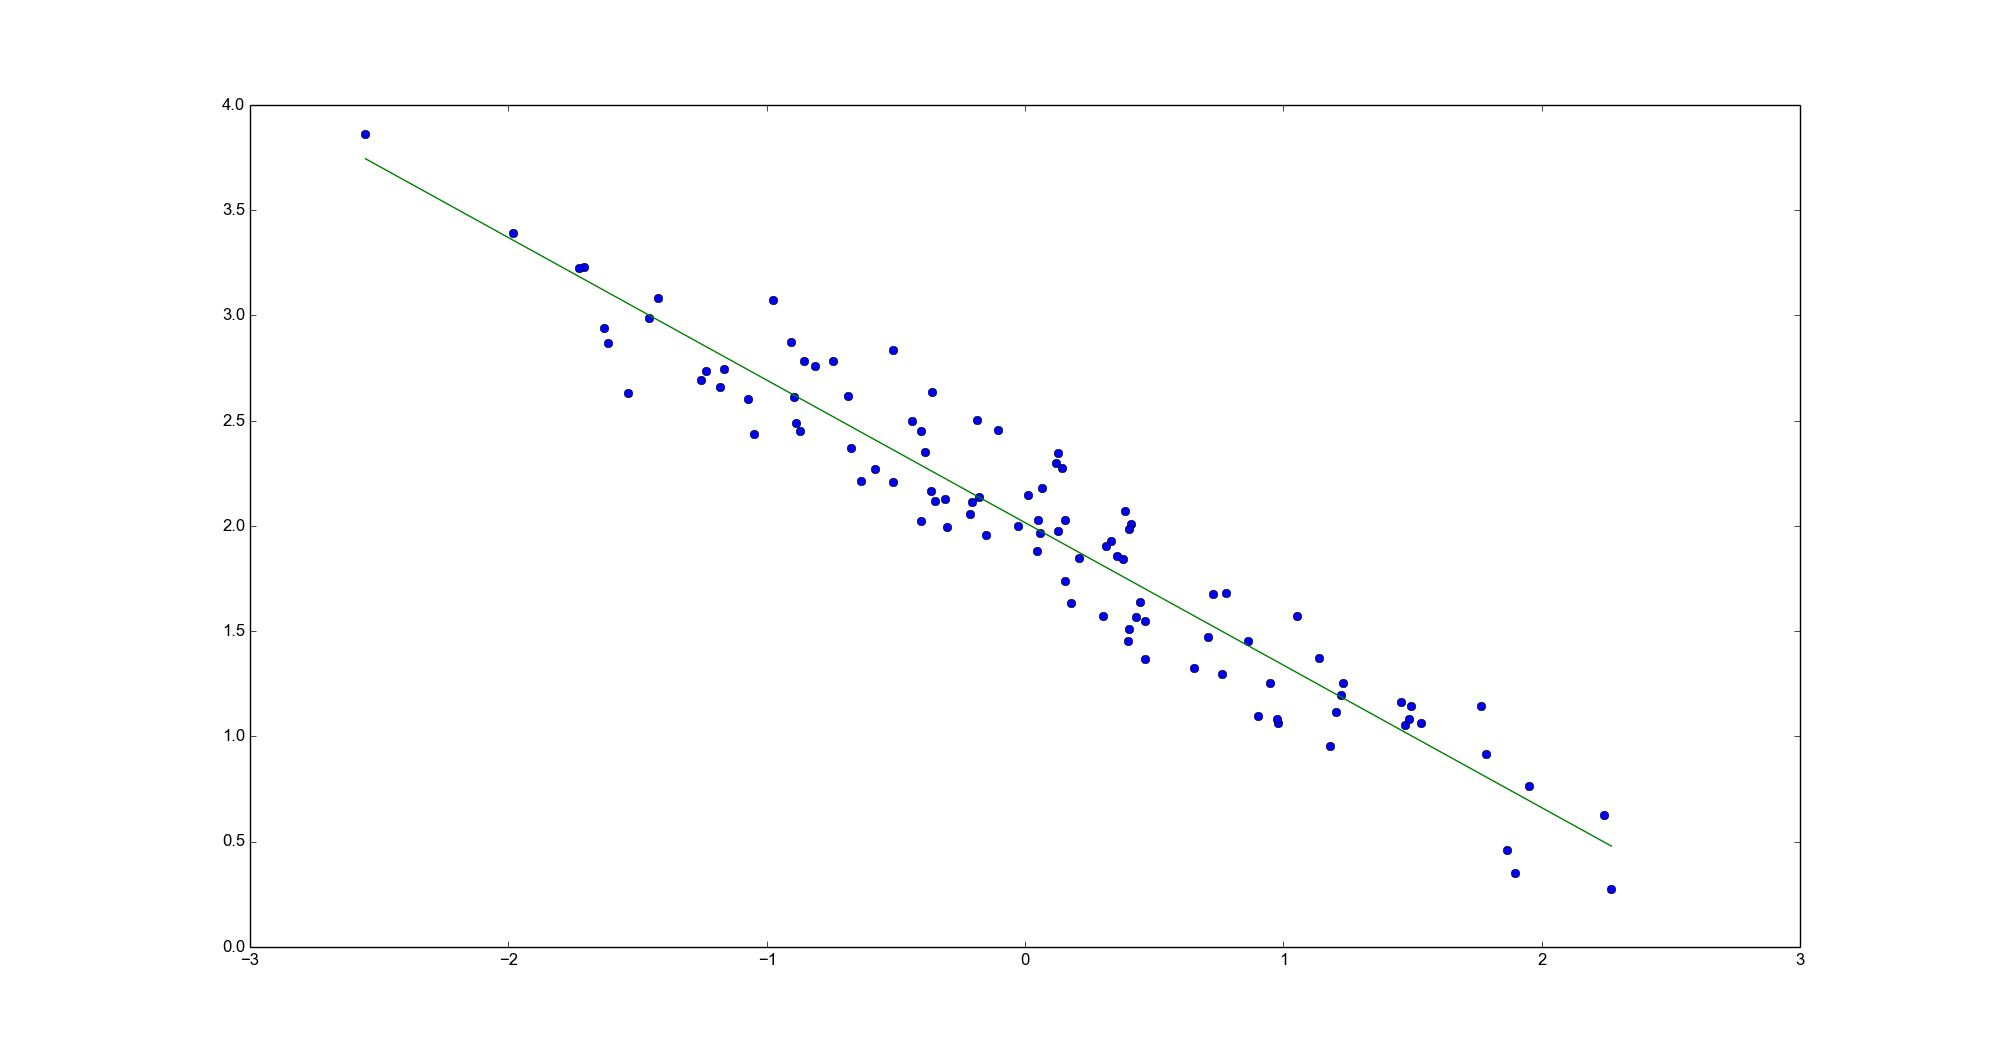
\includegraphics[width=0.8\paperwidth]{figure_1}}

Файл \verb$linregress_plot.py$:
\lstinputlisting[language=Python]{../linregress_plot.py}

\section{Пояснение}
За основу был взят и разобран код программы из раздела Исходный код условия задания.

Исходный код доступен по ссылке:

\href{https://github.com/SvichkarevAnatoly/Course-Python-Bioinformatics/tree/master/bioseq7}{https://github.com/SvichkarevAnatoly/Course-Python-Bioinformatics/tree/master/bioseq7}

\section{Исходный код}
Файл \verb$test_code7.py$:
\lstinputlisting[language=Python]{../test_code7.py}
\end{document} % Конец документа
